\documentclass{article}
\usepackage{hyperref}
\usepackage{longtable}
\usepackage{graphicx}
\usepackage{booktabs}
\usepackage{pdfpages}
\usepackage{float}
\usepackage{ragged2e}
\usepackage{placeins}
\usepackage{caption}
\usepackage{array}
\usepackage{enumitem}
\usepackage{titlesec}
\setcounter{secnumdepth}{4}
\titleformat{\paragraph}
{\normalfont\normalsize\bfseries}{\theparagraph}{1em}{}
\titlespacing*{\paragraph}
{0pt}{3.25ex plus 1ex minus .2ex}{1.5ex plus .2ex}
\title{draft_design}
\author{Caden Roberts}
\date{March 2025}

\begin{document}
\begin{titlepage}
    \centering
    \vfill
    {\Huge \bfseries Project Documentation 3\par}
    \vspace{1.5cm}
    {\Huge
        Akash Srinivasan \par \ \par
        Caden Roberts \par \ \par
        Jhovanny Uribe \par \ \par
        Andy Vo \par \ \par
        Ethan Cesario \par \ \par
        Aliyaa Islam \par \ \par
    }
    \vspace{1cm}
    {\Huge \bfseries Mar 11 2025\par}
    \vspace{1.5cm}
    \href{https://github.com/jhovuribe/Physical-Therapy-Hand-Rehabilitation-Device/}{\Huge \bfseries Github}
\end{titlepage}

\section{\bf{-----Cover Page-----}}


\section{\bf{-----Front Matter-----}}
\section{Executive Summary}

\section{Ethics Statement}
We reference: \href{https://www.apta.org/siteassets/pdfs/policies/codeofethicshods06-20-28-25.pdf}{The Code of Ethics for the Physical Therapist} \\ \\ 
With our physical therapy hand device we aim to address treatment for those who would
benefit from remote commitment to treatment[2][3], adapting to modern trends to benefit
therapists[6] and clients[7] and serving those without consistent access to therapy[8].
\begin{itemize}
\item Principle 2: Physical therapists shall be trustworthy and compassionate in addressing the
rights and needs of patients and clients.
\item Principle 3: Physical therapists shall be accountable for making sound professional judgments.
\item Principle 6: Physical therapists shall enhance their expertise through the lifelong acquisition
and refinement of knowledge, skills, abilities, and professional behaviors.
\item Principle 7: Physical therapists shall promote organizational behaviors and business practices
that benefit patients and clients and society.
\item Principle 8: Physical therapists shall participate in efforts to meet the health needs of people locally, nationally, or globally.
\end{itemize}

\section{Table of Contents}


\section{\bf{-----Body-----}}
\section{Background}

\subsection{Personas}
\subsubsection{End User}
\begin{longtable}{|p{0.3\textwidth}|p{0.7\textwidth}|}
    \caption{User Persona: Mark} \label{table:user_persona} \\
    \hline
    \multicolumn{2}{|c|}{\textbf{End User}} \\ 
    \hline
    \endfirsthead

    \hline
    \multicolumn{2}{|c|}{\textbf{End User} (continued)} \\ 
    \hline
    \endhead

    \hline
    \multicolumn{2}{|r|}{\textit{Continued on next page}} \\ 
    \hline
    \endfoot

    \hline
    \endlastfoot

    
\includegraphics[width=0.25\textwidth]{guy.jpg} & \textbf{Mark, 36 yrs old} \\ 
    \hline
    \textbf{Context} &
    \begin{itemize}
        \item Worked IT desk job for 12 years
        \item Has one kid and two cats
        \item Enjoys spending time with family
        \item Carpal tunnel syndrome caused from typing most of the day on his computer
    \end{itemize} \\
    \hline
    \textbf{Goals} &
    \begin{itemize}
        \item Wants to start stretching hands to make it better as the pain is debilitating, and he really values being active with his family and pets
    \end{itemize} \\
    \hline
    \textbf{What does this entail} &
    \begin{itemize}
        \item He struggles to do the hand exercises prescribed from his doctor as he forgets to
        \item The device will help him be consistent
    \end{itemize} \\
    \hline
\end{longtable}



\begin{longtable}{|p{0.3\textwidth}|p{0.7\textwidth}|}
    \caption{User Persona: Samantha} \label{table:user_persona_samantha} \\
    \hline
    \multicolumn{2}{|c|}{\textbf{End User}} \\ 
    \hline
    \endfirsthead

    \hline
    \multicolumn{2}{|c|}{\textbf{End User} (continued)} \\ 
    \hline
    \endhead

    \hline
    \multicolumn{2}{|r|}{\textit{Continued on next page}} \\ 
    \hline
    \endfoot

    \hline
    \endlastfoot

    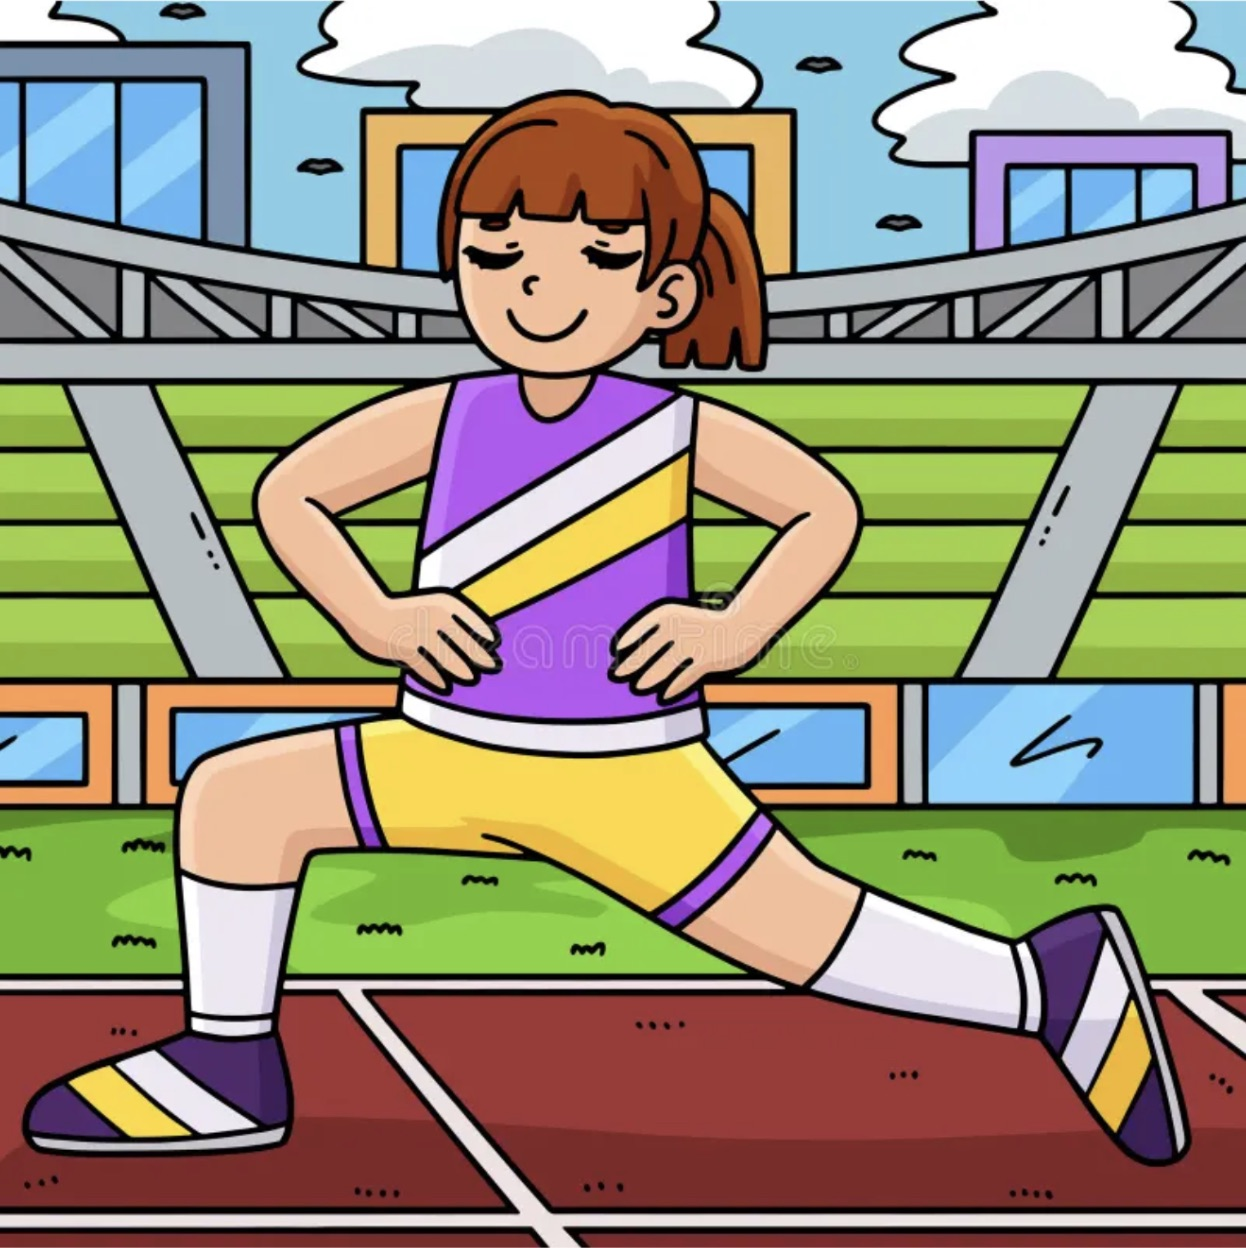
\includegraphics[width=0.25\textwidth]{girl.jpeg} & \textbf{Samantha, 25 yrs old} \\ 
    \hline
    \textbf{Context} &
    \begin{itemize}[leftmargin=*]
        \item Weekend yoga instructor and passionate barista
        \item Enjoys hiking, taking care of her plants, and spending time with friends
        \item Got into car accident and injured hand; lost a lot of strength and mobility because of prolonged cast duration
    \end{itemize} \\
    \hline
    \textbf{Goals} &
    \begin{itemize}[leftmargin=*]
        \item Remain consistent to regain hand mobility
    \end{itemize} \\
    \hline
    \textbf{What does this entail} &
    \begin{itemize}[leftmargin=*]
        \item Struggles with progressing and sticking to physical therapy routine due to active/busy schedule
        \item Stiff/weak joints, time sensitive to regain strength and mobility
        \item Will allow her to progress without losing progress
    \end{itemize} \\
    \hline
\end{longtable}


\begin{longtable}{|p{0.3\textwidth}|p{0.7\textwidth}|}
    \caption{User Persona: Tom} \label{table:user_persona_tom} \\
    \hline
    \multicolumn{2}{|c|}{\textbf{End User}} \\ 
    \hline
    \endfirsthead

    \hline
    \multicolumn{2}{|c|}{\textbf{End User} (continued)} \\ 
    \hline
    \endhead

    \hline
    \multicolumn{2}{|r|}{\textit{Continued on next page}} \\ 
    \hline
    \endfoot

    \hline
    \endlastfoot

    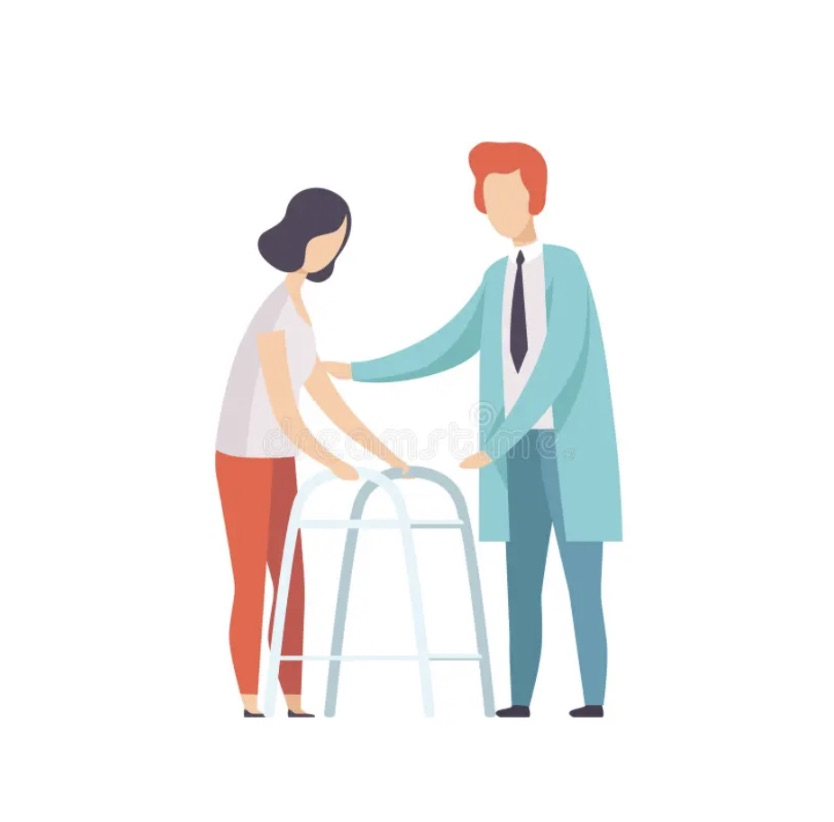
\includegraphics[width=0.25\textwidth]{tom.jpeg} & \textbf{Tom, 42 yrs old} \\ 
    \hline
    \textbf{Context} &
    \begin{itemize}[leftmargin=*]
        \item Physical therapist 
        \item Passionate about helping his clients the best he can
    \end{itemize} \\
    \hline
    \textbf{Goals} &
    \begin{itemize}[leftmargin=*]
        \item Be able to prescribe exercises and track progress remotely with potentially stubborn clients
        \item Retain clients who otherwise would cancel therapy altogether
    \end{itemize} \\
    \hline
    \textbf{What does this entail} &
    \begin{itemize}[leftmargin=*]
        \item Understands that clients have a hard time making it to appointments and not everyone can afford to see him often
    \end{itemize} \\
    \hline
\end{longtable}


\subsubsection{Clients}

\begin{longtable}{|p{0.3\textwidth}|p{0.7\textwidth}|}
    \caption{Client: Insurance Company} \label{table:client_insurance} \\
    \hline
    \multicolumn{2}{|c|}{\textbf{Client}} \\ 
    \hline
    \endfirsthead

    \hline
    \multicolumn{2}{|c|}{\textbf{Client} (continued)} \\ 
    \hline
    \endhead

    \hline
    \multicolumn{2}{|r|}{\textit{Continued on next page}} \\ 
    \hline
    \endfoot

    \hline
    \endlastfoot

    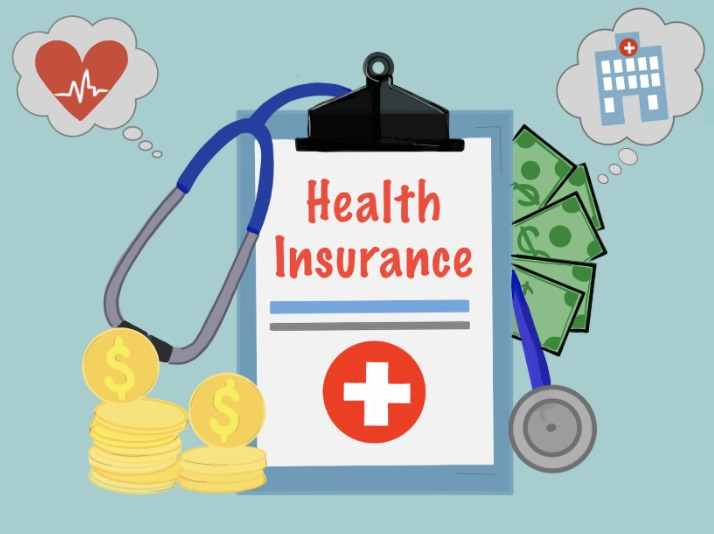
\includegraphics[width=0.25\textwidth]{insurance.jpeg} & \textbf{Insurance Company} \\ 
    \hline
    \textbf{Context} &
    \begin{itemize}[leftmargin=*]
        \item Mid-size health insurance company 
        \item For-profit company
        \item Wants to buy product to provide a service at a cheaper price
        \item Increase retention rate for provided service
    \end{itemize} \\
    \hline
    \textbf{Goals} &
    \begin{itemize}[leftmargin=*]
        \item To provide affordable healthcare to the average person
        \item Allow more accessibility to physical therapy exercises
    \end{itemize} \\
    \hline
    \textbf{What does this entail} &
    \begin{itemize}[leftmargin=*]
        \item Replacing physical therapy visits
        \item Increasing more End Users to have access to in-person therapy meetings
    \end{itemize} \\
    \hline
\end{longtable}

\section{Problem Definition}

\subsection{Need and Goal Statements}
\subsubsection{Need Statement}
Physical therapy for hand rehabilitation is a time- and cost-intensive process with limited at-home alternative option.
\subsubsection{Goal Statement}
We aim to make hand rehabilitation less time and cost intensive by providing an at home option for hand therapy.

\subsection{Design Objectives}
Design a cost-effective solution that is user-friendly and streamlines the rehabilitation process.
\begin{longtable}{|l|l|l|}
    \caption{Design Objectives and Targets} \label{tab:design_objectives} \\
    \hline
    \textbf{Design Objective} & \textbf{Unit} & \textbf{Target/Range} \\ \hline
    \endfirsthead

    \hline
    \textbf{Design Objective} & \textbf{Unit} & \textbf{Target/Range} \\ \hline
    \endhead

    \hline
    \multicolumn{3}{|r|}{\textit{Continued on next page}} \\ \hline
    \endfoot

    \hline
    \endlastfoot

    Visits & Number of visits & 10\%--50\% less \\ \hline
    Device Cost & Dollars & \textgreater{} \$1440 \\ \hline
    Accessibility & Minutes & Greater than session time \\ \hline
    Weight & lbs & \ \textless{} 2 lbs \\ \hline
    % Add more rows as needed
\end{longtable}
\section{Concepts Considered}
\subsection{Brainstorm}
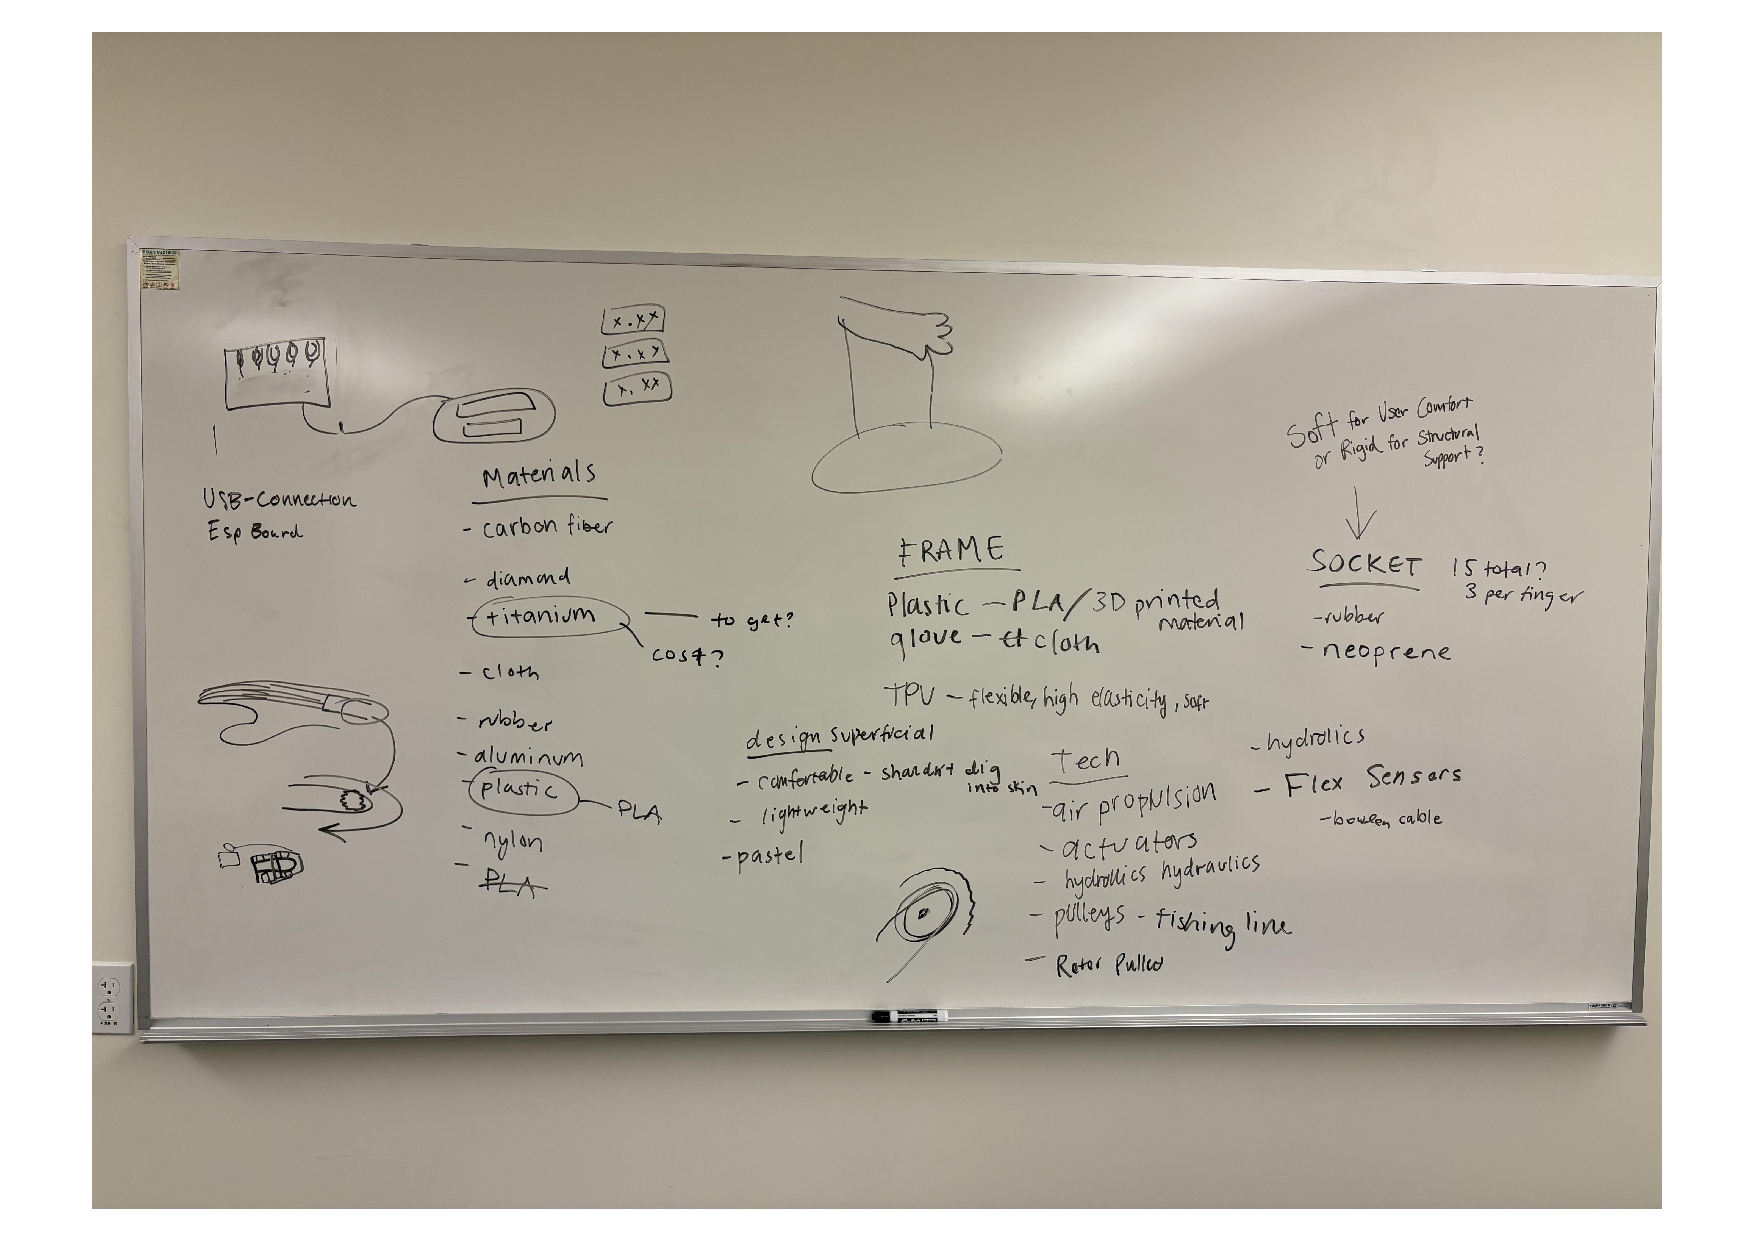
\includepdf[pages=-]{brainstorm.pdf}
\subsection{6-3-5 Method}
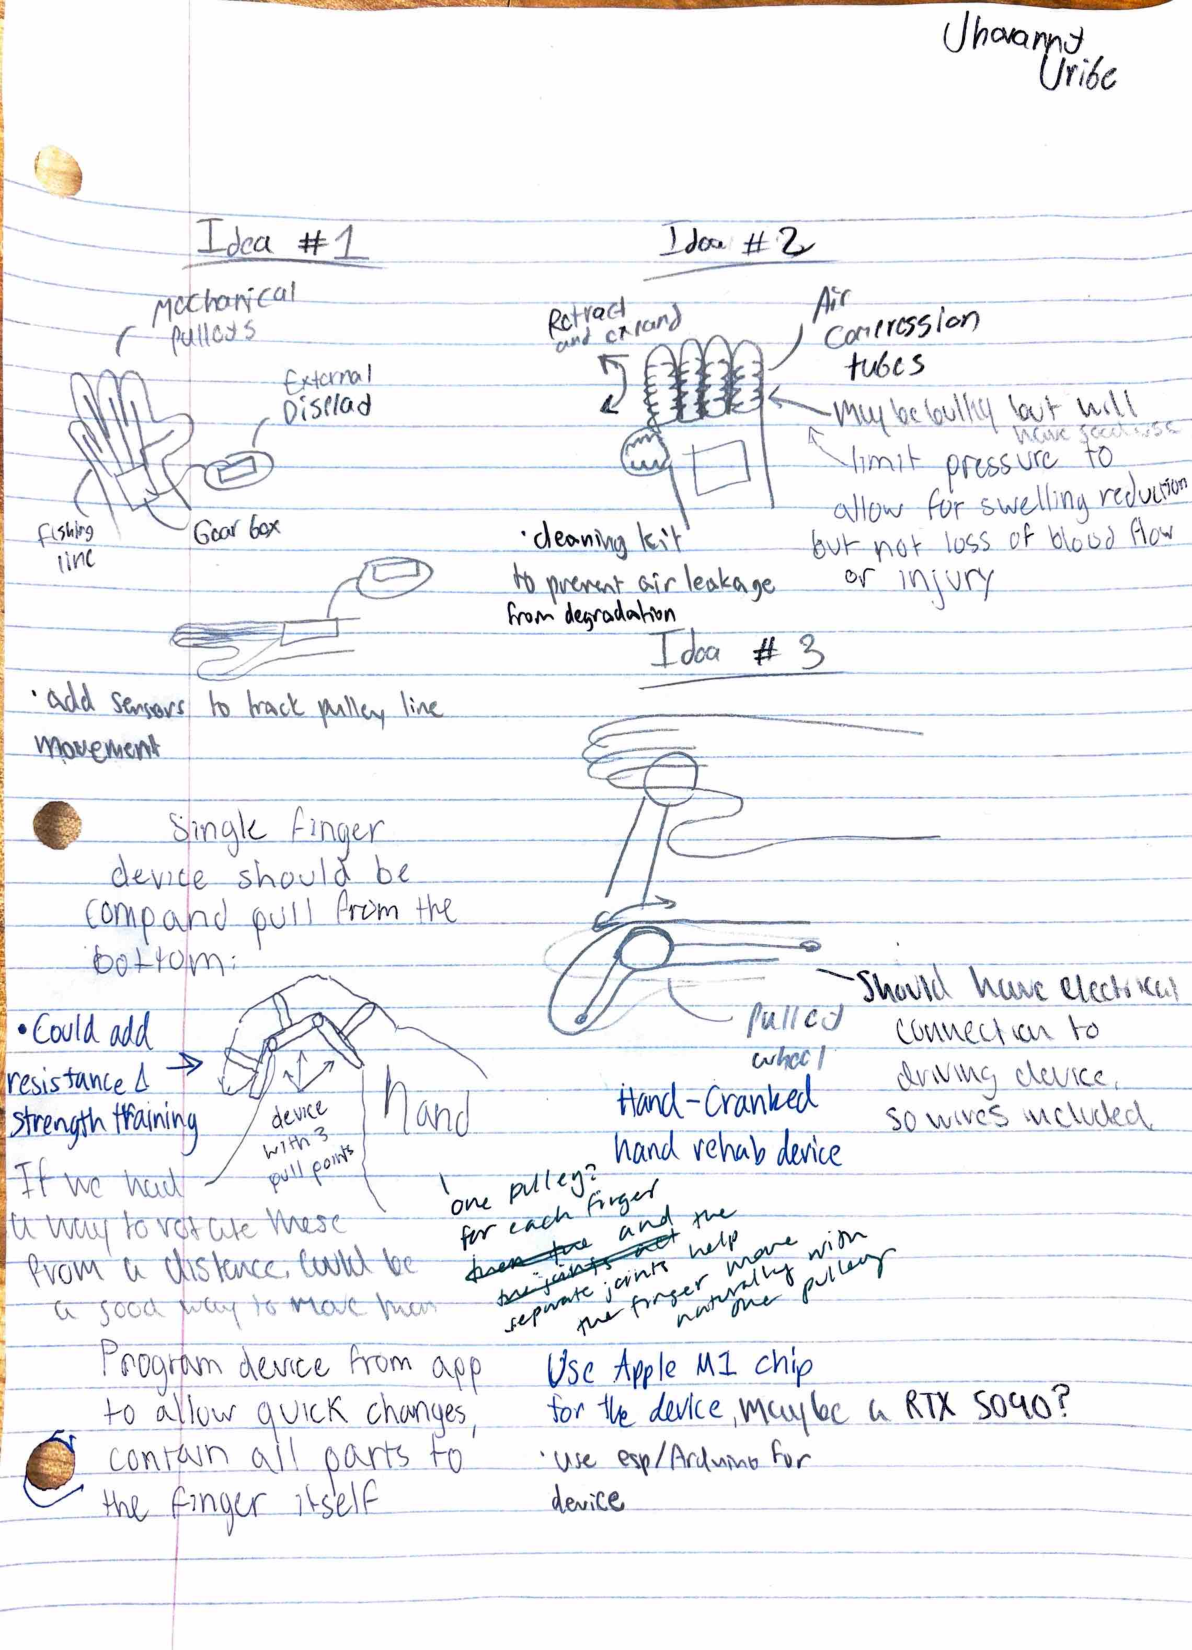
\includepdf[pages=-]{635_Designs.pdf}
\subsection{Morphological Chart}
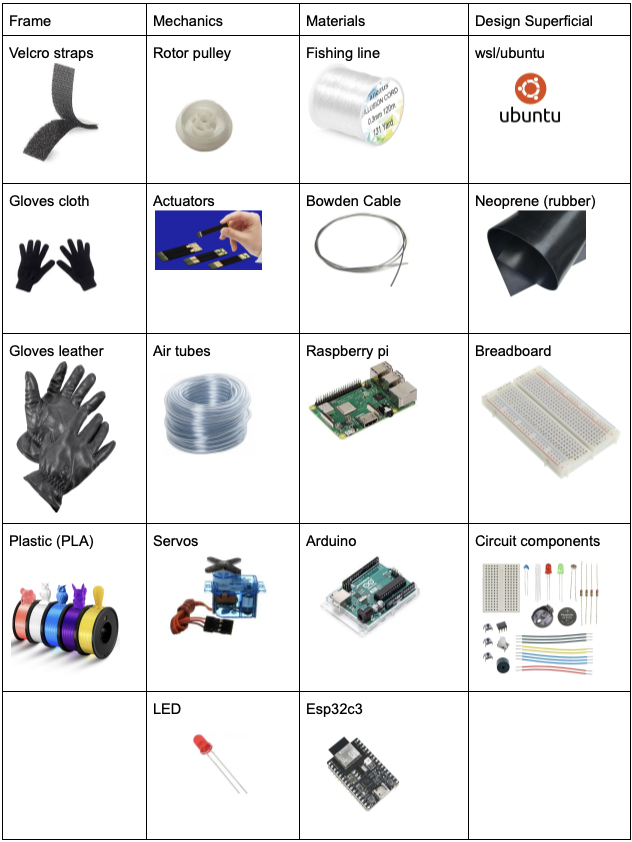
\includegraphics[width=12cm]{morpho.png}
\subsection{Mind Map}
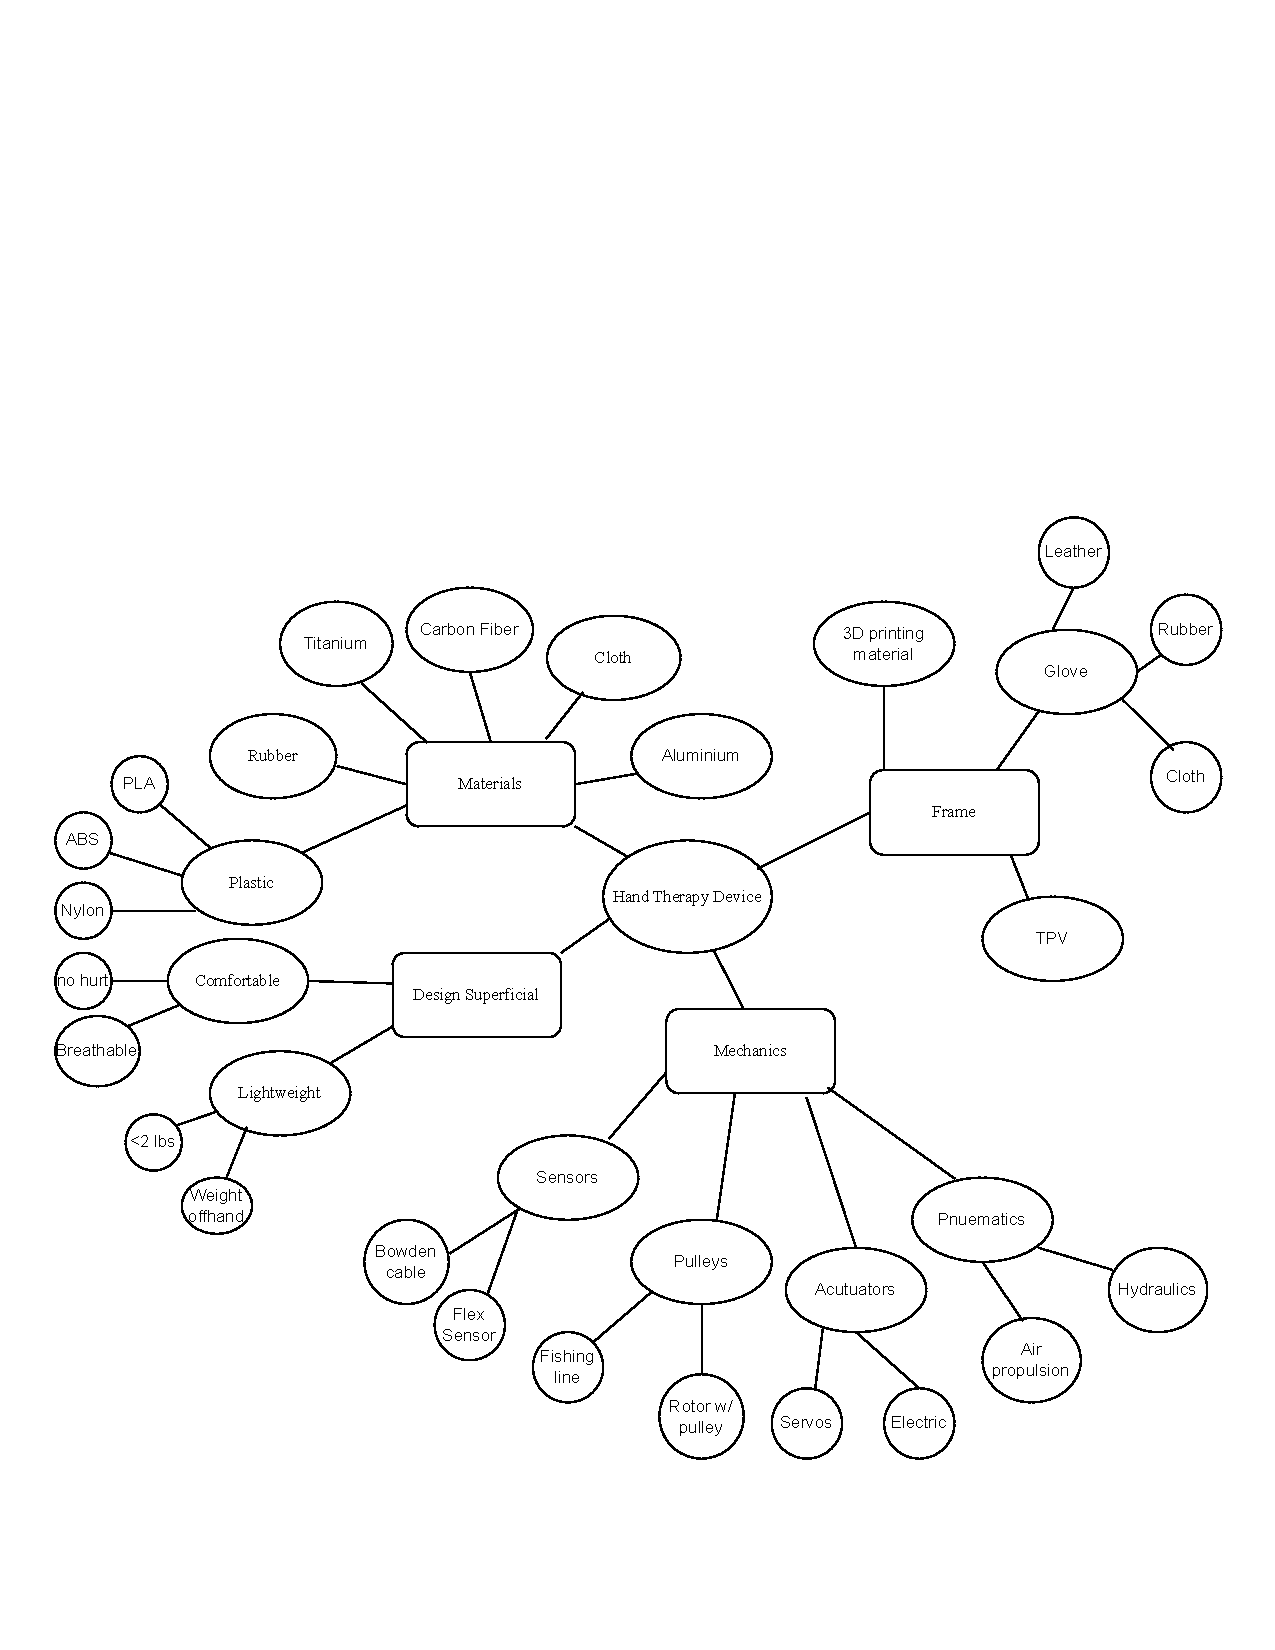
\includepdf[pages=-]{Mindmap.pdf}

\section{Concept Selection}

\subsection{Decision Table}
\begin{table}[h]
    \noindent\hspace{-4.5cm}
    \small
    \begin{tabular}{l c | c c | c c | c c}
        \toprule
        \textbf{Criteria} & \textbf{Weight (\%)} & \multicolumn{2}{c|}{\textbf{Design 1 (Attached Fingers)}} & \multicolumn{2}{c|}{\textbf{Design 2 (Prosthetic Hand)}} & \multicolumn{2}{c}{\textbf{Design 3 (Pneumatic)}} \\
        \cmidrule(lr){3-4} \cmidrule(lr){5-6} \cmidrule(lr){7-8}
        & & Raw & Weighted & Raw & Weighted & Raw & Weighted \\
        \midrule
        Wearability (person) & 20 & 8 & 160 & 7 & 140 & 7 & 140 \\
        Cost & 30 & 9 & 270 & 6 & 180 & 3 & 90 \\
        Damage Likelihood (device) & 10 & 8 & 80 & 6 & 60 & 5 & 50 \\
        Power Consumption & 5 & 10 & 50 & 8 & 40 & 6 & 30 \\
        Weight & 15 & 9 & 135 & 5 & 75 & 4 & 60 \\
        Functionality & 20 & 6 & 120 & 9 & 180 & 10 & 200 \\
        \midrule
        \textbf{Total} & & & 815 & & 675 & & 570 \\
        \bottomrule
    \end{tabular}
\end{table}

\begin{table}[h]
    \centering
    \begin{tabular}{l c}
        \toprule
        \textbf{Criteria} & \textbf{Weight (\%)} \\
        \midrule
        Wearability & 20 \\
        Cost & 30 \\
        Damage Likelihood & 10 \\
        Power Consumption & 5 \\
        Maintenance & 15 \\
        Weight & 20 \\
        \bottomrule
    \end{tabular}
\end{table}

\section{Detail of Design}
Majority of Document

\subsection{Free format description of design}
Include diagrams, schematics, wire-frames, etc.
Be reasonably detailed but remember this is not yet complete

\section{Economic Analysis}

\subsection{Design for Manufacture and Assembly}
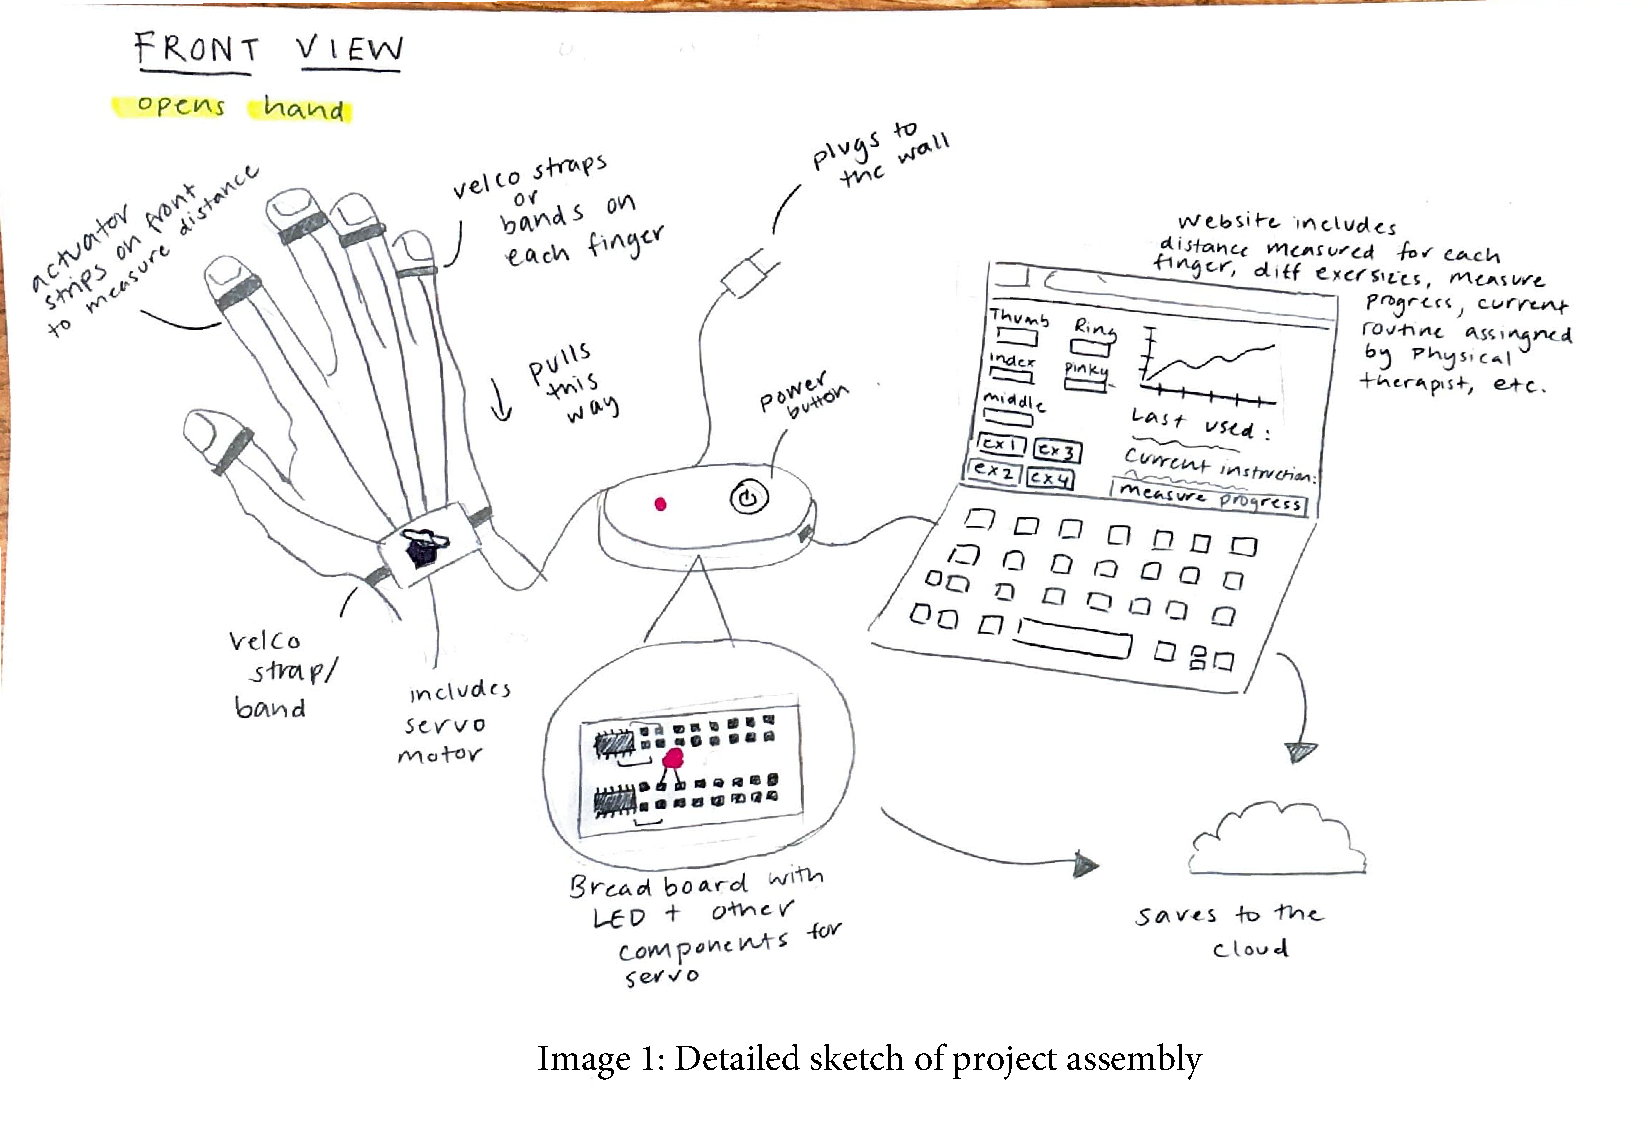
\includepdf[pages=-]{sketch-merged.pdf}

\subsection{Life Cycle Assessment}
\subsubsection{Goal and Scope Definition}
\paragraph{Objective}
The LCA aims to assess the environmental footprint of the Thera-Hand rehabilitation device, considering its:
\begin{itemize}
\item Energy consumption (power supply, servos, ESP32).
\item Material usage (PLA, rubber, fishing line, sensors).
\item Manufacturing and transportation impact.
\item End-of-life disposal/recycling feasibility.
\end{itemize}
\paragraph{Functional Unit}
A single Thera-Hand device is assumed to be used for 2 years before replacement.
\paragraph{System Boundaries}
This LCA includes:
\begin{itemize}
\item Raw Material Extraction – Plastics, rubber, and electronics production.
\item Manufacturing and Assembly – 3D printing, PCB production, servo motor production.
\item Transportation – From manufacturing to users.
\item Use Phase – Power consumption during operation.
\item End of Life – Disposal, recycling, or potential reuse.
\end{itemize}
\subsubsection{Inventory Analysis}
\paragraph{Material Composition and Impact}
\begin{table}[h]
    \hspace*{-3.5cm}
    \centering
    \begin{tabular}{|l|l|l|}
        \hline
        \textbf{Component} & \textbf{Material} & \textbf{Environmental Impact} \\ 
        \hline
        Frame \& Housing & PLA (3D printed) & Low-carbon footprint, biodegradable under specific conditions \\ 
        \hline
        Sensors & Flexible PCB, resistive materials & Electronic waste, difficult to recycle \\ 
        \hline
        Actuators (Servos) & Plastic, copper wiring & High-energy manufacturing, limited recyclability \\ 
        \hline
        Power Supply & Electronic components, metal & Requires responsible e-waste disposal \\ 
        \hline
        Wiring \& Fishing Line & Copper wiring, nylon & Small footprint, but non-biodegradable \\ 
        \hline
    \end{tabular}
    \label{tab:material_composition}
\end{table}
\paragraph{Energy Consumption(Use Phase)}
Based on prior power consumption estimates:
\begin{table}[h]
    \hspace*{-2.2cm}
    \centering
    \begin{tabular}{|l|c|c|c|}
        \hline
        \textbf{Component} & \textbf{Power Consumption (W)} & \textbf{Usage per day (hours)} & \textbf{Annual Energy (kWh)} \\ 
        \hline
        ESP32 & 1.25W & 2 & 0.91 kWh \\ 
        \hline
        5 SG90 Servos & 6.25W (idle) / 16.25W (peak) & 1 & 5.93 kWh \\ 
        \hline
        Sensors \& LED & 0.15W & 2 & 0.11 kWh \\ 
        \hline
        \textbf{Total Estimate} & $\approx$ 7.65W - 17.65W & - & 6-7 kWh/year \\ 
        \hline
    \end{tabular}
    \caption{Comparison: This is equivalent to a low-power LED bulb running for ~3 months.}
    \label{tab:energy_consumption}
\end{table}
\subsubsection{Impact Assessment (Environmental)}
\paragraph{Manufacturing:}
\begin{itemize}
\item Electronics production (ESP32, sensors, servos) has the highest carbon footprint.
\item 3D printing (PLA) requires energy but has a relatively low impact compared to metals.
\end{itemize}
\paragraph{Use Phase:}
\begin{itemize}
\item Low electricity consumption (~6-7 kWh/year) makes it energy-efficient.
\end{itemize}
\paragraph{End-of-Life Considerations:}
\begin{itemize}
\item PLA parts are biodegradable in industrial composting but not in landfills.
\item Servos, wiring, and PCBs require responsible e-waste recycling.
\end{itemize}
\subsubsection{Interpretation and Recommendations}
\paragraph{Key Findings}
\begin{itemize}
    \item Low Energy Consumption: Thera-Hand is energy-efficient in use.
    \item Minimal Carbon Footprint for PLA: The frame is eco-friendly, but plastics must be disposed
of properly.
    \item E-Waste Challenge: Sensors, servos, and the ESP32 must be recycled properly.
    \item Transportation Impact: If shipped globally, the CO$_2$ footprint increases.
\end{itemize}
\paragraph{Recommendations}
\begin{itemize}
    \item Optimize 3D Printing Material: Use recycled PLA or biodegradable TPU to reduce waste.
    \item E-Waste Collection Plan: Offer a recycling take-back program for electronics.
    \item Reduce Servo Impact: Use low-power or energy-efficient servos if possible.
    \item Sustainable Packaging: Use biodegradable or recycled materials for packaging.
\end{itemize}

\subsubsection{Conclusion}
\begin{itemize}
\item Thera-Hand is a low-energy, partially sustainable device.
\item The biggest environmental concern is e-waste disposal of sensors and servos.
\item Efforts to recycle electronic components and use sustainable materials can improve its
eco-friendliness.
\end{itemize}

\section{Outstanding Issues}


\section{\bf{-----Appendices-----}}
\section{Models and Simulations}

\section{Decision Table Inputs}

\section{Test Plan}
\subsection{Ability to be turned on/off}
The device should have the ability to be turned off separately from being unplugged.

\subsubsection{Goal} The device should be able to be turned on and off while still connected to a direct power source.

\subsubsection{External Factors} Make sure the power connection is stable and not under loaded.

\subsubsection{Equipment} Hand device with external bank, Power Source.

\subsubsection{Steps}
\begin{enumerate}
\item The device should not be connected to any person.
\item The device should be connected to an AC stable power supply of at least 120 Volts. A common wall socket is preferred.
\item Load any basic exercise and wait more than 10 seconds.
\item Turn off the device by pressing the power button on the box connected to the wall. Make sure to press the power button before the exercise has ended.
\item Observe and measure the time it takes the device to stop moving.
\item Repeat steps 3-5 multiple times with different exercises.
\end{enumerate}

\subsection{Ability to download/save metrics}
Data should be stored and sent remotely after each exercise is completed.

\subsubsection{Goal} The device should be able to remotely send data to an external device that can store data.

\subsubsection{External Factors} Unstable power supply, unstable internet connection, and connectivity issues.

\subsubsection{Equipment} Hand device with external bank, Power Source, Separate device connected to the Internet and connected to the device.

\subsubsection{Steps}
\begin{enumerate}
\item Plug the device into a stable 120 Volts AC power supply, preferably a wall outlet.
\item Load the exercise onto the device and begin the workout. Preferably a short workout routine.
\item Connect the therapist's device to a stable internet connection.
\item Pair the device to a therapist's computer, allowing it to download and store the device's workout data.
\item Start the workout and wait for it to finish.
\item Observe the download of the device.
\end{enumerate}

\subsection{Weight}
Determine the weight of the device that is on the hand. Under two pounds.

\subsubsection{Goal} The device should weigh less than 2 pounds or 1 kilogram.

\subsubsection{External Factors} The scale should be accurate enough to detect under five pounds and should be zeroed before use.

\subsubsection{Equipment} Hand device without external bank, small scale.

\subsubsection{Steps}
\begin{enumerate}
\item Unplug the device from the power bank and computer.
\item Place the device on the scale. The glove should be dry and empty. Strings should be attached from servos to the fingers.
\end{enumerate}

\subsection{Accuracy of repetition counting}
The device should be tested to report as many repetitions as are being performed. We need to know the degree of error of our data.

\subsubsection{Goal} The device should count the repetitions performed ideally with perfect accuracy.

\subsubsection{External factors} The device should be properly calibrated to recognize when a full range of motion repetition has occurred.

\subsubsection{Equipment} Hand device with external bank, Power Source, Separate device connected to the internet and connected to the device.

\subsubsection{Steps}
\begin{enumerate}
\item Plug the device into a 120 Volt AC outlet.
\item Turn the device on and begin a basic squeezing exercise, beginning with fingers outstretched, then fully contracting all fingers to the center of the palm (must touch to be counted as a rep), and finally outstretch all fingers again.
\item While the device records repetitions, manually count how many repetitions occur until the time is over.
\item Compare the number of repetitions the device reports to the number of repetitions observed.
\end{enumerate}

\subsection{Individual controllability}
Each finger should be able to operate independently of any other finger.

\subsubsection{Goal} Verify that each finger is independently programmable and movable.

\subsubsection{External factors} Individual anatomy and flexibility of those being tested.

\subsubsection{Equipment} Hand device with external bank, Power Source, Separate device connected to the internet and connected to the device.

\subsubsection{Steps}
\begin{enumerate}
\item Plug the device into a 120 Volt AC outlet.
\item First, turn the device on and verify that each finger can be pulled in individually.
\item Lastly, check that each finger can individually be extended back out.
\end{enumerate}

\subsection{Resting state}
The device should return to a resting state after the completion of each exercise.

\subsubsection{Goal} The device should be verified to return to a neutral state after each exercise is completed.

\subsubsection{External factors} Someone’s anatomy or flexibility may prevent a typical “neutral” resting state.

\subsubsection{Equipment} Hand device with external bank, Power Source, Separate device connected to the internet and connected to the device.

\subsubsection{Steps}
\begin{enumerate}
\item Plug the device into a 120V AC outlet.
\item Turn the device on and begin a basic squeezing exercise, beginning with fingers outstretched, then fully contracting all fingers to the center of the palm (must touch to be counted as a rep), and finally outstretch all fingers again.
\item After completion of the exercise, verify that the device has returned to its neutral resting state.
\end{enumerate}

\subsection{Full Range of Motion on each finger}
The device should be able to move in the full range of motion for each finger. Determine through flex sensor data in the amount of flexion (degrees).

\subsubsection{Goal} The device should demonstrate flexion within the expected biomechanical range (0-90 for DIP, 0-100 for PIP, 0-90 for MCP, depending on finger). Deviation beyond 2.5\% of standard human range to be flagged for recalibration. If the device does not meet the expected range, adjustments in control algorithms and mechanical design may be necessary.

\subsubsection{External factors} Ambient temperature variations, Device vibrations and mechanical inconsistencies, Any potential latency in response times.

\subsubsection{Equipment} Glove with integrated flex sensors, Voltage divider circuit with known resistor (? ohms), Arduino, Computer for data logging and visualization.

\subsubsection{Steps}
\begin{enumerate}
    \item Mount the device securely and ensure proper calibration of flex sensors.
    \item Record natural rest position of each finger.
    \item Actuate each finger from full extension to full flexion.
    \item Record flex sensor data at key points of movement (0, 45, 90, etc.).
    \item Repeat the process for each finger, ensuring consistency.
\end{enumerate}

\subsection{Ability to fit on a common hand}
The device should be able to fit securely and comfortably on common hand sizes, using straps for adjustability.

\subsubsection{Goal} The device should securely fit common hand sizes without excessive gaps or pressure points. The adjustable straps should allow for a customized fit without discomfort. If fit issues arise, modifications to strap length, padding, or buckle placement may be necessary.

\subsubsection{External factors} Impact of movement on strap security. Any noticeable discomfort due to prolonged wear.

\subsubsection{Equipment} Robotic/assistive hand device with straps for adjustability. 3D hand model (male/female). Measuring tools for assessing gaps and pressure points (ruler, measuring tape, etc.). User feedback for qualitative comfortability assessment.

\subsubsection{Steps}
\begin{enumerate}
    \item Prepare the hand models and device with adjustable straps. Ensure straps are at their default adjustment before each trial.
    \item Measure the circumference of each hand model at the middle of the hand and forearm.
    \item Place the device on each hand model and secure it using the straps. Adjust the straps for a snug but comfortable fit.
    \item Record strap tension using measuring tape and pressure sensors.
    \item Conduct subjective assessment for comfort and stability.
\end{enumerate}

\subsection{Durability of the device}

\subsubsection{Goal} The device should maintain functional integrity for at least 100,000 flexion cycles without significant degradation. The structural components should withstand typical impact forces without catastrophic failure. Environmental exposure should not lead to material breakdown or loss of functionality. If durability issues arise, material selection, mechanical design, or protective coatings may need revision.

\subsubsection{External factors} Effects of prolonged use on mechanical performance. Environmental factors leading to premature material failure.

\subsubsection{Equipment} Robotic/assistive hand device. Mechanical testing rig for repeated flexion cycles. Load cell sensors to measure stress and strain. Environmental chamber for temperature and humidity variations. Impact testing apparatus for drop and shock resistance.

\subsubsection{Steps}
\begin{enumerate}
    \item Mount the device on a mechanical testing rig.
    \item Calibrate sensors to measure force, stress, and performance degradation.
    \item Record initial material integrity and functionality metrics.
    \item Subject each finger mechanism to repeated flexion cycles (minimum 100,000 cycles).
    \item Monitor for signs of wear, stiffness, or failure.
    \item Drop the device from various heights onto different surfaces. 
    \item Assess structural damage and continued operability.
    \item Expose the device to temperature fluctuations (-10 Celsius to 50 Celsius) and high humidity.
    \item Evaluate material degradation and operational stability.
\end{enumerate}

\section{Test Results}

\begin{table}[H]
    \hspace*{-1 cm}
    \centering
    \begin{tabular}{|c|c|p{8cm}|}
        \hline
        \textbf{Name(s)} & \textbf{Date/Location} & \textbf{Tests} \\
        \hline
        & & \textbf{Test 1:} Did the power turn off? (Yes/No) \\
        \hline
        & & \textbf{Test 2:} Was data remotely sent? (Yes/No) \\
        \hline
        & & \textbf{Test 3:} Weight: (kg/lbs) \\ 
        \hline
        & & \textbf{Test 4:} What accuracy were the repetitions counted to? (\%) \\
        \hline
        & & \textbf{Test 5:} How many fingers were individually controllable? (0-5) \\
        \hline
        & & \textbf{Test 6:} Did the device return to a resting state? (Yes/No) \\
        \hline
        & & \textbf{Test 7:} Full Range of Motion on each finger? (Yes/No) \\
        \hline
        & & \textbf{Test 8:} Ability to fit on common hand? (Yes/No) \\
        \hline
        & & \textbf{Test 9:} Device Durability acceptable? (Yes/No) \\
        \hline
    \end{tabular}
    \caption{Test Log}
    \label{tab:test_log}
\end{table}

\end{document}
